

In the following, we present the informal 
specification that Fraunhofer FOKUS derived from analysing the 
implementation of \bitwalker.

\subsection{Basic concepts}

First we introduce various terms that we will use in our informal specifications.
In particular, we distinguish between \emph{bit streams} and \emph{bit sequences}.

\begin{itemize}
\item
A \emph{bit stream} is an array containing elements of type \verb"uint8_t".

\item
If \inl{a} is the starting address of a bit stream and
if all pointers \inl{a+[0..n-1]} are \emph{valid} in the sense
of the \isoc standard (cf.~\cite[\S~6.5.3.2(4)]{ISO:C99}),
then we refer to \inl{a} as a \emph{valid bit stream of length \inl{n}}.

\item 
A bit stream of length $n$ contains $8n$ bits.

\item 
A bit stream can be indexed both by array indices
and \emph{bit indices}.

Figure~\ref{fig:bitstream-indices} shows the difference between 
array indices (bottom row) and bit indices (top row) in a bit stream.
The two bit indices, 0~and~14,
mark bit positions in the first and second array element, respectively.

\begin{figure}[hbt]
\begin{center}
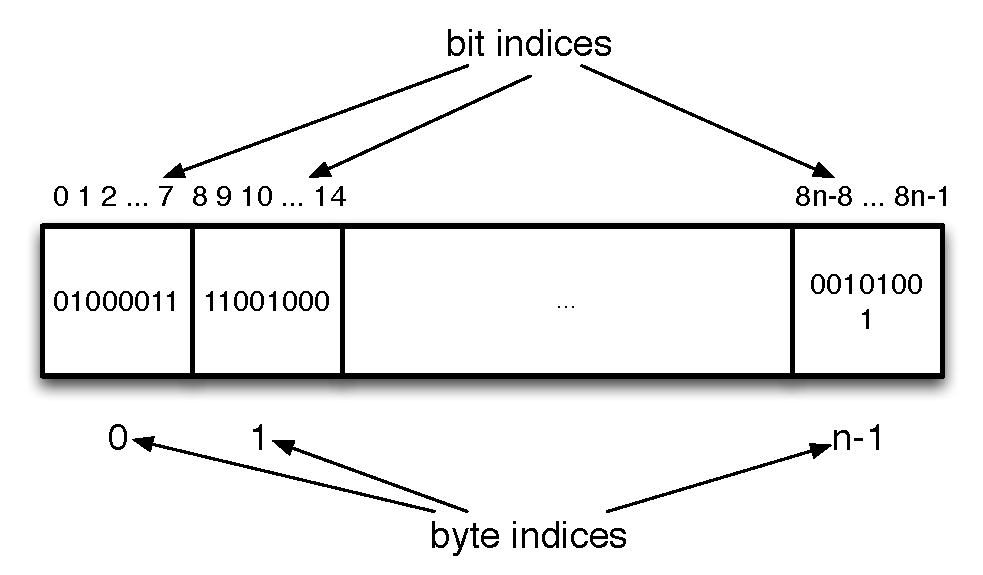
\includegraphics[width=0.65\textwidth]{figures/byte-and-bit-indices.pdf}
\caption{\label{fig:bitstream-indices} Byte indices and bit indices in a bit stream}
\end{center}
\end{figure}


\item 
The C~programming language neither provides a type \emph{bit}
nor does it support random access to the bits of a bit stream.
In order to access the $i$-th bit of a bit sequence one typically
has to first access the byte with index $j = i/8$ and then access the 
bit $k = i \% 8$ within this byte.
Note that in Figure~\ref{fig:bitstream-indices} 
bytes and bits are indexed in increasing order, starting from the \emph{left}.
In big-endian mode, however, bits are indexed from the \emph{right}.
For example, to access the $k$-th bit (from the left) of a byte \inl{a} one can
shift this byte to the right by $7-k$ bits and then extract the now
rightmost bit by performing a bit-wise \emph{and} with the value~1
%
\begin{verbatim}
   (a >> (7-k)) & 1        // get the k-th left-most bit of a
\end{verbatim}

\item
A \emph{bit sequence} is a consecutive sequence of bits within a bit stream
as represented in Figure~\ref{fig:bitsequence}.
\begin{figure}[hbt]
\begin{center}
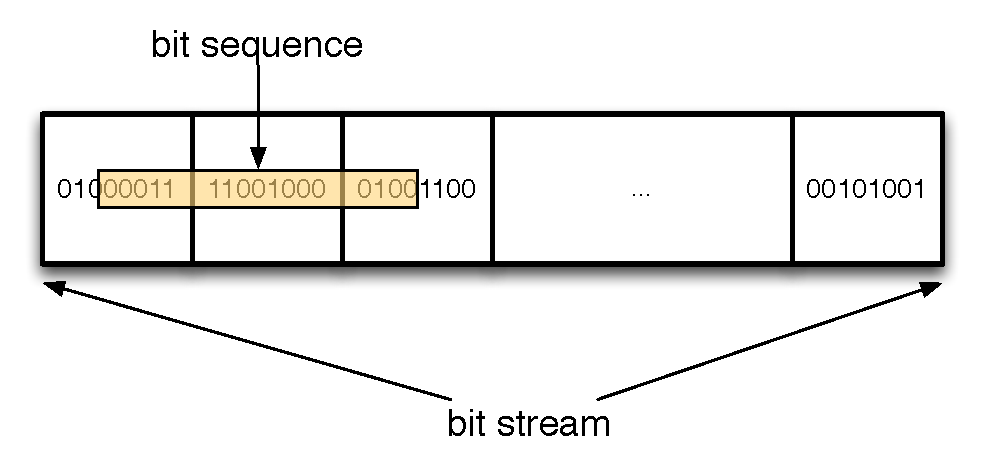
\includegraphics[width=0.65\textwidth]{figures/bit_sequence.pdf}
\caption{\label{fig:bitsequence} A bit sequence within a bit stream}
\end{center}
\end{figure}

A bit sequence is given by the position of its first bit (a bit index in the bit stream)
and its \emph{length}, that is, the number of bits it contains.

\item

A bit sequence that starts at bit index $p$ and has
length $l \geq 0$ is considered \emph{valid} (with respect to a bit stream of length $n$)
if the following conditions are satisfied
\begin{align*}
  0 &\leq p < 8n \\
  0 &\leq p + l \leq 8n
\end{align*}

Note that only the bits with indices $p \leq i < p + l$ are to be accessed
but not the bit with index~$p+l$.

\end{itemize}

We assume that the C-types \inl{unsigned int} and \inl{int}, which
are used in the implementation to represent indices, counting and error codes,
have a width of~32~bits.
We point this out here because we conducted the verification on a platform with
these characteristics.

As an aside, MISRA-C discourages the use of ``generic'' integer types
such as \inl{int} and \inl{unsigned int} and recommends the use of integer types whose names
contain the exact width.

